\chapter{Wstęp}
W ostatnich latach zarysowuje się coraz większa potrzeba wdrażania systemów informatycznych w celu usprawniania funkcjonowania firm. Występuje wiele ich rodzajów: CRM (ang. Customer Relationship Managment) - wspomagające zarządzanie relacjami z klientami, ERP (ang. Enterprise Resource Planning) – wspomagające zarządzanie i planowanie zasobami firmy czy też BPM (ang. Business Process Managment) – wspomagające zarządzanie procesami biznesowymi. Wprowadzanie systemów informatycznych do firm może wywoływać różnorodne efekty: techniczne (związane z zastosowaniem techniki komputerowej: zwiększenie szybkości przetwarzania informacji, wzrost dokładności przetwarzania, wzrost szczegółowości informacji, poprawa bezpieczeństwa poufnych informacji) ekonomiczne (związane pośrednio ze wzrostem efektywności i szybkości podejmowania decyzji), organizacyjne (przede wszystkim związane są z usprawnieniami struktury organizacyjnej i procesów zachodzących w przedsiębiorstwie: podniesienie sprawności obiegu dokumentów, eliminacja zbędnej pracy administracyjnej, poprawa koordynacji zadań, eliminacja błędów), socjopsychologiczne (związane przede wszystkim z rozszerzeniem zakresu komunikacji pomiędzy pracownikami, usprawnieniem systemu ocen pracowniczych, polepszeniem kultury organizacyjnej). \cite{EfektyZasSys}

Utworzenie systemu informatycznego dla dużych firm i instytucji nie stanowi zadania trywialnego. Banki, uczelnie lub urzędy charakteryzują się często stosunkowo złożoną strukturą organizacyjną oraz panują w nich skomplikowane procesy wewnętrzne. Powstaje wówczas problem z formalnym opisem danej jednostki – niezbędnym do utworzenia sprawnie działającego, spełniającego wymagania klienckie systemu informatycznego. Bardzo istotnym elementem jest wówczas stosowanie odpowiedniej metodyki, która pozwoli na usystematyzowane podejście do projektowania tego rodzaju systemów. 

\section{Cel pracy}
Podstawowym celem pracy jest opracowanie nowej metodyki projektowania systemów o architekturze korporacyjnej, która będzie opierała się na wykorzystaniu języka SoaML. Dotychczas utworzono już podobne metodyki, jednakże żadna nie była w stanie w pełni sprostać wszystkim wymaganiom stawianym przez problematykę projektowania systemów o architekturze korporacyjnej. 

Projekt metodyki będzie się opierał na wybraniu najmocniejszych stron oraz pominięciu wad istniejących metodyk. Autor pracy podejmie również próbę wdrożenia innowacyjnych elementów do zaprojektowanej metodyki, które będą miały na celu usprawnienie procesu projektowania architektury korporacyjnej.

Zaprojektowana metodyka zostanie również poddana weryfikacji i testom przy tworzeniu niewielkiego systemu bankowego.

\section{Założenia dla pracy}
Oprócz założenia głównego dla pracy – utworzenie własnej metodyki projektowania architektury korporacyjnej z zastosowaniem SoaML- postawiono kilka innych, które powinna realizować:
\begin{itemize}
\item{zdefiniowanie architektury korporacyjnej oraz wyjaśnienie terminów z nią powiązanych,}
\item{omówienie obecnych metodyk wykorzystywanych do projektowania architektury korporacyjnej,}
\item{omówienie języków wykorzystywanych do projektowania architektury korporacyjnej,}
\item{weryfikacja koncepcji autorskiej metody przy wdrożeniu przykładowego systemu bankowego.}
\end{itemize}

\chapter{Charakterystyka architektury korporacyjnej}
\section{Wstęp}
\section{Czym jest architektura korporacyjna?}
\section{Definicje głównych pojęć związanych z architekturą korporacyjną}
\section{Korzyści z wdrożenia architektury korporacyjnej}
\section{Podejście do budowy architektury korporacyjnej}
\section{SOA}
\subsection{Czym jest SOA?}
Trudno o jednoznaczną definicję SOA (ang. Service Oriented Architecture – architektura zorientowana na usługi). Definicja SOA jest subiektywna, zależna od punktu widzenia. Z perspektywy biznesowej (odbiorcy usług) rozumieć ją można jako zestaw usług wspierających realizację procesów biznesowych. Odnosząc się do SOA z perspektywy IT widzimy ją jako infrastrukturę potrzebną do dostarczenia tych usług.
	
Organizacja W3C (World Wide Web Consortium) podjęła próbę zdefiniowania SOA. Według niej SOA to zbiór komponentów, które mogą być wywoływane, i których interfejsy mogą być publikowane i wykrywane (ang. A set of components which can be invoked, and whose interface descriptions can be published and discovered).

Z kolei firma IBM definiuje SOA jako podejście do budowania systemów rozproszonych dostarczających funkcjonalność aplikacji w postaci usług, które mogą być udostępniane aplikacjom zewnętrznym lub innym usługom. \cite{PlatIntGor}

Istnieje również manifest SOA, który głosi, że orientacja na usługi kształtuje punkt widzenia na to co chcemy wykonać, a SOA stanowi typ architektury, który jest wynikiem takiej orientacji. (ang. Service orientation is a paradigim that frames what you do. Service-oriented architecture (SOA) is a type of architecture that results from applying service orientation). \cite{SOAManifestoOrg}

SOA sama w sobie nie jest jednakże żadną konkretną architekturą. Nie można jej traktować jako produkt lub tylko zbiór określonych rozwiązań technologicznych. SOA to przede wszystkim sposób myślenia – strategia, której naturalna realizacja jest reprezentowana przez usługi. \cite{SOAsdj102009,SOAwJBBC} SOA stanowi pewnego rodzaju paradygmat, który prowadzi do określonej architektury. \cite{SOAsdj102009}
	
Mianem usługi w SOA określa się zbiór funkcjonalności pewnej aplikacji, który jest udostępniany jako interfejs. \cite{SOAawidptas} Organizacja OASIS definiuje usługę w SOA jako mechanizm udostępniający jedną lub więcej funkcji, do których dostęp jest zapewniany przez zalecany interfejs i wykonywany zgodnie z ograniczeniami i politykami określanymi przez opis usługi (ang. A mechanism to enable access to one or more capabilities, where the access is provided using a prescribed interface and is exercised consistent with constraints and policies as specified by the service description). Operacje, zdefiniowane w interfejsie dostarczają funkcji biznesowych operując na obiektach biznesowych. Ponadto owe usługi są dostępne poprzez sieć.[JSOAcookkb] 

\subsection{Historia SOA}
Określenia „SOA” lub „Architektura zorientowana na usługi” zostały po raz pierwszy wykorzystane w pracy naukowej analityka z firmy Garnter Yefim V. Natis w dniu 12 kwietnia 1996 roku. 

\subsection{Budowa SOA}
SOA wprowadza nowe podejście do budowy i zarządzania infrastrukturą informatyczną. Adaptacja SOA wiąże się z reguły ze zmianami w wielu obszarach funkcjonowania firmy. Ściśle wiąże się z panującymi w niej procesami biznesowymi i wymaga odpowiedniego dostosowania.[SOAPAIesdasb] 

Systemy opierające się na SOA składają się z zestawu aplikacji biznesowych pogrupowanych w niezależne komponenty, które komunikują się ze sobą wymieniając usługi. [SOAwJBBC, SOAidntech]. 

\begin{figure}[h!tbp]
\begin{centering}
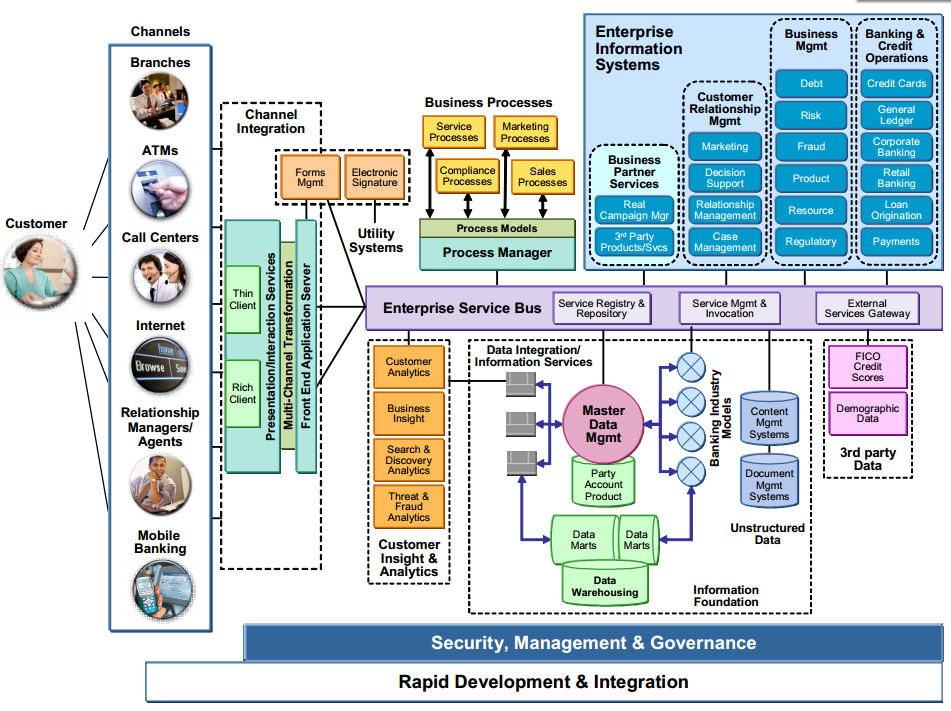
\includegraphics[width=14cm]{img/soa_arch.png}
\caption[Przykładowa architektura SOA.]{Przykładowa architektura SOA. \cite{AnRTeqq}}\label{soa_arch}
\end{centering}
\end{figure}
Rys. [PRZArchSOA] Przykładowa budowa systemu SOA.
Komponenty te można traktować jako tzw. „czarne skrzynki”. Klient korzystający z usługi otrzymuje jedynie interfejs. Implementacja udostępnionych metod nie jest dla niego istotna.
Rozwiązania stosowane w SOA pomagają zapanować nad złożonością systemu. Podstawowa budowa SOA opiera się z reguły na szynie ESB (ang. Enterprsie Service Bus) integrującej poszczególne usługi. ESB jest efektywnym środkiem komunikacji w SOA. Pomaga uwolnić się od sieci powiązań „każdy z każdym”. [SOAidntech] Odpowiada za przesyłanie komunikatów do odpowiednich komponentów. Rozbudowa systemu polega na dołączaniu nowych usług do szyny integracyjnej. 
	
Komunikaty zanim zostaną wysłane do punktu docelowego często poddawane są transformacjom i odpowiedniemu dostosowaniu za pomocą mediacji (ang. mediations) na ESB. Przetworzony komunikat odpowiada formie jakiej oczekuje dostawca usługi.
	
Rejestr SOA (ang. SOA registry) stanowi centralny punkt informacyjny na temat sposobu dostępu, definicji, reguł, bezpieczeństwa i innych danych wymaganych do wykorzystania usług udostępnionych w danym środowisku SOA. Zawiera informacje gdzie poszczególne komponenty SOA są umieszczone. Na jego podstawie ESB potrafi prawidłowo przekierowywać żądanie usługi i ewentualną odpowiedź, a aplikacje i usługi korzystające z usług składowych potrafią skonstruować jej prawidłowe wywołanie. [SOAidntech, SOAfddum]
	
Istotnym elementem w systemach typu SOA jest repozytorium (ang. SOA repository). Stanowi on centralny „magazyn” dla elementów składowych usług takich jak: kod źródłowy, zestawy instalacyjne, specyfikacja itp. Repozytorium usług jest tworzone i wykorzystywane głównie na etapie projektowania usług. [SOAidntech]

\subsection{Podstawowe zasady SOA}
Systemy SOA mogą być bardzo różnorodne. SOA nie narzuca konkretnych technologii, a jej realizacja może odbywać się na wiele sposobów. Komunikacja mędzy komponentami w SOA może wykorzystywać różne kanały komunikacji: WS, HTTP, HTTPS, LDAP, FTP, IMAP, JMS, RMI. Budowa systemu SOA może wykorzystywać szynę integracyjną ESB lub broker (można również łączyć wiele szyn ESB ze sobą lub łączyć broker’y z ESB). Mimo tej dużej dowolności istnieje zestaw zasad, na których powinien opierać się każdy system SOA.
\begin{itemize}
\item{luźne powiązania - powiązania odnoszą się do połączeń lub relacji między poszczególnymi elementami. [SOAterlprD] Termin „luźne powiązania” (ang. Loose Coupling) stanowi jeden z fundamentów SOA. [SOAsdj102009] Odwołuje się do sposobu w jaki komponenty SOA współpracują ze sobą.  Zasada „luźnych powiązań” promuje niezależną konstrukcję i ewolucję usług. Każdy z komponentów może pracować autonomicznie wykonując określone czynności. Pracując razem, wymieniają między sobą komunikaty i mogą realizować to co jest zwykle możliwe przez duże, monolityczne aplikacje. „Luźne powiązania” pozwalają również na łatwą dekompozycję komponentów i wykorzystywanie ich do innych celów. [SOAterlprD, SOAidntech]}
\item{interoperacyjność - interoperacyjność (ang. interoperability) opiera się na współpracy pomiędzy systemami. Zapewnienie interoperacyjności jest kolejną bardzo istotną zasadą, o której należy pamiętać tworząc systemy SOA. W miarę rozwoju poszczególnych systemów (np. poprzez dodawanie nowych komponentów) problem integracji staje się coraz trudniejszy do rozwiązania. Należy już na etapie projektowania ograniczać do minimum oraz wybierać odpowiednie protokoły, które dany system będzie obsługiwał. [SOAsdj102009]}
\item{composability - zasada composability jest związana z zachowaniem odpowiednich relacji między komponentami. Systemy, które podążają za ta zasadą cechują się możliwością łączenia swoich komponentów w różne kombinacje w celu spełnienia postawionych wymagań. Umiejętność efektywnego komponowania usług z już istniejących jest kluczowym wymogiem dla osiągnięcia niektórych z najbardziej podstawowych celów przy tworzeniu systemów opierających się na architekturze zorientowanej na usługi. [SOAterlprD]}
\item{reużywalność - każda tworzona usługa powinna zachowywać zasadę reużywalności (ang. reusability).  Opiera się ona na takim projektowaniu usług, aby była możliwość wielokrotnego jej wykorzystania do tworzenia kolejnych usług. [SOAsdj102009]}
\item{kontraktowość usług - każda usługa powinna mieć zdefiniowany kontrakt (ang. service contract), który zawierany jest każdorazowo pomiędzy usługą, a jej konsumentem. Wyrażane są przez nie cele i możliwości danej uslugi. [SOAterlprD] W kontraktach znajdują się również opisy informacji oferowanych  i oczekiwanych przez usługi. [SOAinfoq10]}
\item{abstrakcyjność - zasada abstrakcji (ang. abstraction) zakłada, że kontrakty usług mogą zawierać jedynie niezbędne informacje i mogą udostępniać jedynie te informacje, które są w nich zdefiniowane. Zasada ta podkreśla potrzebę ukrycia przez usługi tak wielu informacji jak to tylo możliwe. [SOAterlprD]}
\item{autonomiczność usług - autonomia usługi (ang. service autonomy) jest kolejnym paradygmatem projektowania systemów typu SOA. Termin ten odwołuje się do usług o podwyższonej niezależności od środowisk wykonawczych. [SOAsrvautoWCSS] Usługa powinna mieć możliwość podmiany środowiska wykonawczego z lekkiego prototypowego (ang. lightweight prototype) do pełnowymiarowego (ang. full-blown), w którym są już uruchomione inne usługi odwołujące do niej. Zgodnie z zasadą autonomii każda z usług może być wdrażana, wersjonowana i zarządzana niezależnie od innych. [SOAinfoq10]}
\item{wykrywalność usług - zasada wykrywalności usług (ang. services discoverability) polega na tym, że usługi powinny być opisywane za pomocą meta danych w takich sposób, aby były efektywnie wyszukiwane, przetwarzane i interpretowane zarówno w czasie projektowania jak i wykonywania. [SOAinfoq10, SOAsrvautoWCSS]}
\item{spójność i ziarnistość usług - interfejsy usług w systemach SOA powinny być tak zaprojektowane, aby wiązały tylko określony zbiór wymagań biznesowych. \cite{SOAsdj102009} Należy zadbać o optymalną ziarnistość interfejsów dla obsługiwanych typów i rozmiarów danych (ziarnistość danych wejściowych i wyjściowych), wartości biznesowej oraz funkcjonalności (domyślna i parametryzowana ziarnistość funkcjnonalności). [SOAdefgranaaImp]}
\item{bezstanowość usług - zasada bezstanowości usług (ang. Services statelessness) odwołuje się do minimalizacji użycia zasobów i ograniczania się do przechowywania i przetwarzania tylko absolutnie niezbędnych informacji.  [SOAsrvautoWCSS ] Usługa nie może być w stanie przetrzymywać informacji o wcześniejszych żądaniach klienta. Każda z informacji powinna być odizolowana od innych. Skuteczne stosowanie zasady bezstanowości może znacząco zwiększyć wydajność rozwiązania oraz zmniejszyć współbieżne działanie usług. \cite{SOAsdj102009}}
\item{enkapsulacja - enkapsulacja (ang. Encapsulation) stanowi jedną z podstawowych zasad poprawnego projektowania systemów typu SOA. Zapewnienie odpowiedniej hermetyzacji dla usług sprowadza się do ukrywania szczegółów konfiguracyjnych oraz implementacyjnych danej usługi.}
\end{itemize}

\section{Adaptacja SOA w architekturze korporacyjnej}

\chapter{Metodyki projektowania rozwiązań w architekturze usługowej}
\section{Wstęp}
\section{RUP4SOA}
\subsection{Czym jest RUP?}
RUP (ang. \textit{Rational Unified Process}) stanowi proces  wytwarzania oprogramowania oparty na iteracjach. Metodyka ta została zdefiniowana przez grupę Rational Software (przejętą przez firmę IBM w roku 2003). 

RUP zapewnia zdyscyplinowane podejście do przydzielania zadań i obowiązków w ramach rozwoju organizacji. Celem podstawowym tej metodyki jest dostarczenie wysokiej jakości oprogramowania spełniającego potrzeby użytkowników końcowych w zgodzie z harmonogramem i ramami budżetowymi.
\cite{RUPIntRat} Stanowi przede wszystkim bardzo duży zbiór praktyk, który może być dostosowywany i rozszerzany w celu jak najlepszego dopasowania się do danej organizacji. Charaktertystyczne dla metody jest rozwój sterowany przypadkami użycia (ang. \textit{Use Case Driven Development}).\cite{RUPMartFow}

W RUP można wyróżnić poszczególne fazy:
\begin{itemize}
\item{faza początkowa (ang. \textit{inception}) – wstępne określenie wymagań, ryzyka, kosztu, harmonogramu, a także architektury systemu,}
\item{faza opracowania (ang. \textit{elaboration}) – ustalenie wymagań (większości przypadków użycia), architektury systemu oraz planu całego procesu wytwarzania systemu,}
\item{faza konstrukcji (ang. \textit{construction}) – tworzenie systemu (kolejnych komponentów), w trakcie następuje oddanie pierwszej (i być może dalszych) wersji użytkownikowi,}
\item{faza przekazania (ang. \textit{transiation}) – system jest przekazywany użytkownikowi, wdrażany, szkoleni są pracownicy obsługi systemu, następuje walidacja i końcowe sprawdzenie jakości.}\cite{RUPIntRat}
\end{itemize}
\subsection{Wykorzystanie RUP w projektowaniu SOA}
RUP4SOA stanowi modyfikację metodyki RUP i dołączono do niej zadania i produkty potrzebne przy projektowaniu rozwiązań w architekturze usługowej. W odróżnieniu od klasycznego RUP, metodyka RUP4SOA opiera się na wyróżnieniu trzech dyscyplin związanych z analizą i projektowaniem:
\begin{itemize}
\item{analiza i projektowanie architektury SOA - przygotowanie architektury SOA zgodnie z wymaganiami,}
\item{analiza i projektowanie kontraktów w architekturze SOA - analizie poddane są procesy integracyjne, związane z dostarczaniem usług i realizacją kontraktów między organizacjami,}
\item{analiza i projektowanie logiki usług SOA - identyfikacja usług w systemach informatycznych w jednostkach, w których wdrażana będzie architektura SOA}
\end{itemize}
Reszta dyscyplin jest analogiczna do metodyki RUP. \cite{PlatIntGor}

W RUP4SOA można wyróżnić poszczególne dyscypliny:
\begin{itemize}
\item {modelowanie biznesowe,}
\item {specyfikacja wymagań,}
\item {analiza i projektowanie architektury SOA,}
\item {analiza i projektowanie kontraktow SOA,}
\item {analiza i projektowanie logiki usług,}
\item {implementacja,}
\item {testowanie,}
\item {wdrożenie,}
\item {zarządzanie zmianą i konfiguracją,}
\item {zarządzanie projektem,}
\item {środowisko.}
\end{itemize}

\section{SOMA}

\chapter{Przegląd języków do projektowania systemów informatycznych o architekturze SOA}
\section{SoaML}
\subsection{Czym jest SoaML?}
\subsection{Główne elementy notacji}
\subsection{Modelowanie z wykorzystaniem SoaML}
\section{ArchiMate}
\section{Inne języki}

\chapter{Opracowanie metody projektowania systemów informatycznych o architekturze SOA}

\chapter{Weryfikacja koncepcji na przykładzie systemu bankowego}
\section{Projektowanie systemu bankowego w oparciu o utworzoną koncepcję}
\subsection{Opis ogólny}
\subsection{Analiza systemu}
\subsection{Implementacja}
\subsection{Proces wdrożenia}
\subsection{Testy}
\section{Cel systemu w odniesieniu do zaprojektowanej koncepcji}
\chapter{Podsumowanie i wnioski}
